\chapter{Performance-Analysis}

Before going into the performance tests itself, it is required to understand some fundamentals about network communication and the anatomy of a \gls{http} request.
\\

\section{Introduction}

"To reduce their design complexity, most networks are organized as a \textbf{stack of layers or levels}, each one built upon the one below it" \cite{kn1}[sec. 1.3.1]. The same holds true for the protocol stack driving the "internet". There exist various models for naming and describing the different layers. In context of the internet usually the "TCP/IP Reference Model" is used \cite{kn1}. This model describes five independent layers, each build upon the next underlying layer. 

Real communication between two systems, i.e. exchange of data, always happens on the lowest layer (the "Physical Layer"). But from a logical point of view, communication happens on each layer between the two systems. Therefore each layer might add a header in front of the data, specifying meta information for its counterpart on the other system. Header data of layers above the current layer is treated as if it would belong to the message itself (see figure \ref{fig:header-layers}).

%\begin{wrapfigure}{r}{.45\textwidth}
\begin{figure}[H]
	\centering
	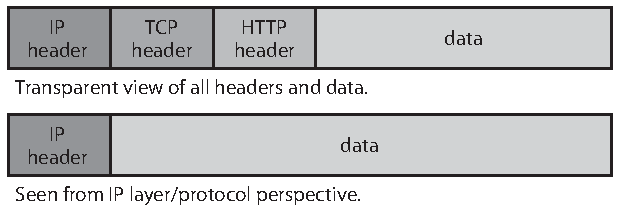
\includegraphics[scale=1]{images/protocol-headers.pdf}
	\caption{Header data for multiple protocol layers (3-5).}
	\label{fig:header-layers}
\end{figure}
%\end{wrapfigure}

Figure \ref{fig:net-layers} shows the five layers of the TCP/IP model with corresponding communication protocols and modules implementing the protocol on the developed test system. On construction of single parameters for a performance benchmark, it needs to be taken into account which parts of the system are effected by this parameter and might influence the results.

%\begin{wrapfigure}{r}{.5\textwidth}
\begin{figure}[H]
	\centering
	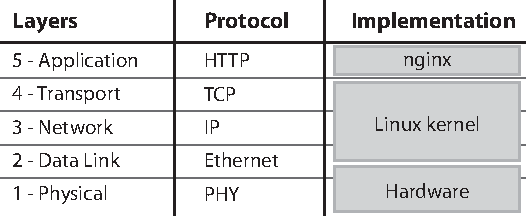
\includegraphics[scale=1]{images/network-layers.pdf}
	\caption{Layers of the network stack with reference to implementing modules.}
	\label{fig:net-layers}
\end{figure}
%\end{wrapfigure}

\subsection{Maximal Transfer Unit (MTU)}
\label{subsec:mtu}

\gls{mtu} is a parameter specifying the maximum size of a single unit transferred over the network in bytes. It is set for a complete network (sender, receiver, intermediate stations), specifying and limiting its capacity to a robust and reliable usage level. When \gls{mtu} values for connected stations differ, the lowest takes effect. 

In Ethernet networks the \gls{mtu} is usually set to 1500 bytes \cite{kn1}. The \gls{mtu} value as used in Linux includes only message data as received by the Ethernet layer. Header data of the Ethernet protocol does not count into this size limit. When messages (including header data of upper layers) exceed the \gls{mtu} size, they are split into multiple packets. In practice this means that for transmitting a single HTTP message (i.e. request or response) two or more \gls{tcp} messages might be required.
\\

\subsection{Transmission Control Protocol (TCP)}

Although \gls{http} is not fixed to be used only with \gls{tcp}; \gls{http} on top of \gls{tcp} on top of \gls{ip} is the most dominant usage combination. This is, because \gls{tcp} provides reliable communication on top of unreliable networks \cite{tcp}. \gls{tcp} accomplishes this by setting up and maintaining a connection. Therefore sending data over TCP consists of three steps: establishing a connection, sending the actual message, closing the connection. To guarantee arrival of sent data, \gls{tcp} works with a handshake protocol between both involved parties for connection state management and acknowledge messages for received packets. 

The overhead of maintaining a connection is the price to be paid for a reliable communication channel between two systems. But it also allows sending more than one message using an already established connection. This comes in handy, when the size of a message exceeds the \gls{mtu} or multiple \gls{http} requests are send to a server (used in persistent HTTP connections, also called "HTTP keep-alive" \cite{http}).

The \textit{Internet Protocol} (IP) introduced so called IP addresses as identifiers for single systems. \gls{tcp} extends this model by port numbers. An application providing services to other systems (i.e. a server) uses one single port, but client applications need to open separate ports for each \gls{tcp} connection. This is required, because \gls{tcp} connections are identified by the four parts "server address", "server port", "client address" and "client port" \cite{tcp}. The TCP header contains two 16 bit fields for source and destination port \cite{kn1}. This leads to a maximum of $2^{16} = 65,536$ concurrently used (open) \gls{tcp} connections on a single client system. This limitation on the capacity of clients needs to be taken into consideration for the design of performance benchmarks. Otherwise observed performance limits might be mistakenly interpreted as limits of the server system \cite{httperf}.
\\

\clearpage
\section{Measuring Web Server Performance}

Pure network performance is often measured as throughput in bits per second. While this gives a great insight in the capabilities of the network, there is no indication as to how many users can be served concurrently by a web server running on the system under test. To gain insights in this performance parameter, dedicated tests on \gls{http} level need to be performed.

A simple method for measuring performance in terms of request throughput is to "send requests to the server at a fixed rate and to measure the rate at which replies arrive" \cite{httperf}. By monotonically increasing the request rate, the server becomes saturated at a certain point. This becomes visible in leveling off reply rates and shows that the server operates at full capacity. \cite{httperf}
\\

\subsection{Tools}

\subsubsection{httperf}

\textit{httperf}\footnote{\url{http://www.hpl.hp.com/research/linux/httperf/}} is a tool developed by David Mosberger and Tai Jin at Hewlett-Packard to specifically measure web server performance \cite{httperf}.

Characteristics of performed tests can be specified by command line arguments to \textit{httperf}. Besides a number of self-explanatory parameters, there are three relevant parameters shaping the actual performance test: \texttt{rate}, \texttt{num-conns} and \texttt{num-calls}.

The \texttt{rate} parameter specifies the rate at which connections are created per second. \texttt{num-conns} specifies the total number of connections to be created during one test run. \texttt{num-calls} specifies the number of requests made over a single TCP connection before it is closed.

A call to \textit{httperf} used for performance tests looks like the following:

\texttt{httperf --timeout=5 --client=0/1 --server=192.168.2.125 --port=80 --uri=/index.html} $\hookleftarrow$ \\
\texttt{--rate=120 --send-buffer=4096 --recv-buffer=16384 --num-conns=3000 --num-calls=3} \\

When executing \textit{httperf} a warning might be displayed:

\texttt{warning: open file limit > FD\_SETSIZE; limiting max. \# of open files to FD\_SETSIZE}

What it basically means is that the process reached the limit of concurrently allowed open file descriptors. This is a per process limit enforced by the \gls{os}. \textit{httperf} is using the \textit{select}\footnote{"\texttt{select}" is an event library provided by the Linux kernel.} module for dealing with network tasks and creates a new file descriptor for every TCP connection. Therefore the limit on open file descriptors limits the number of usable TCP connections by \textit{httperf} and might influence the result of performance tests.

\clearpage
To fix this issue, limits on the current system need to be increased and \textit{httperf} re-compiled. This includes three steps\footnote{The described solution to the FD\_SETSIZE problem was taken from Guillaume Maury: \url{http://gom-jabbar.org/articles/2009/02/04/httperf-and-file-descriptors}.}:

\begin{enumerate}
\item To increase the hard limit of open file descriptors for all users, the following line needs to be inserted (or updated) in \texttt{/etc/security/limits.conf}: "\texttt{* hard nofile 65535}"

\item The value of the pre-compiler constant "\texttt{\_\_FD\_SET\_SIZE}" needs to be increased to \texttt{65535}. It is defined in "\texttt{/usr/include/bits/typesizes.h}". \\
This file might be located in another sub-directory, e.g. "\texttt{/usr/include/x86\_64-linux-gnu/bits/typesizes.h}".

\item \textit{httperf} needs to be re-compiled from source:\\
 \\
\texttt{wget} \url{ftp://ftp.hpl.hp.com/pub/httperf/httperf-0.9.0.tar.gz}\\
\texttt{tar xvzf httperf-0.9.0.tar.gz \&\& cd httperf-0.9.0\\
./configure \&\& make\\
sudo make install}
\end{enumerate}

A useful helper for automating test runs with increasing connection rate is \textit{autobench}\footnote{\url{http://www.xenoclast.org/autobench/}}. It is a Perl script acting as a wrapper around \textit{httperf} and was published by Julian Midgley.
\\

\subsubsection{Custom Scripts}

In addition to accurate engineered test cases using \textit{httperf}, custom scripts were used to generate load on the server. A small Windows console application written in \texttt{C\#}, utilizing the \textit{Task Parallel Library}\footnote{\url{http://msdn.microsoft.com/de-de/library/vstudio/dd460717.aspx}}, turned out to be the most efficient one with best performance characteristics.

This console application is also included in the appendix of this report (see \ref{appendix:csharp-load}).
\\

\subsubsection{Wireshark}

\textit{Wireshark}\footnote{\url{http://www.wireshark.org}} is a network protocol analysis software, which captures all traffic going through a network interface. It especially helps in analyzing and inspecting captured data through its deep knowledge of all common protocols.

It was used in this project for debugging initial problems with the network stack and low-level analysis of performance test parameters.
\\

\section{Tests}

The tests were conducted using \textit{httperf} on a virtual machine running \textit{Ubuntu Linux 12.04}. To proof that the limiting factor during the tests is not this client machine, but the system under test, all tests were also performed against a \textit{Microsoft IIS 7.5} web server instance, which was hosted on a bare metal machine with an \textit{AMD Phenom II X4 965} processor at 3.40 GHz, running \textit{Microsoft Windows 7 Professional} as operating system.

According to statistics of the \textit{HTTP Archive}\footnote{\url{http://httparchive.org/interesting.php\#responsesizes} (as of Dec. 15th 2012)} an average HTML page has a size of about 6 KB. Other content types, like images, stylesheets and script files vary on average between 5 KB and 21 KB. 

Taking this usage pattern of websites into consideration, tests were performed using static files with two sizes: one file having exactly 10 KB (10.240 bytes) from now on referred to as "10K.html" and one very minimal HTML page having just 354 bytes ("index.html"). The major difference between these two files from a "network perspective" is that the small file can be transmitted in two TCP packets, one is used for the HTTP header and one for the actual data (see section \ref{sec:nginx-os-if}), whereas the 10 KB file needs to be split up in 9 TCP packets due to the default \gls{mtu} size of 1500 bytes. A third test-run was performed requesting a file that does not exist. This results in a HTTP response with code "404 -- Not Found". It is a special case, because the response is transmitted in a single TCP packet and no file needs to be read from the file system.

Figure \ref{fig:initial-req} shows request and response rates for all three test cases with an increasing connection rate (20 conn./s to 120 conn./s, step size: 10). On each connection three HTTP requests were made to the respective file. 

On every connection rate level 3,000 connections were opened to obtain reliable results. Therefore each test run included 33,000 connections and up to 99,000 requests.

\begin{figure}[H]
	\centering
	\begin{tikzpicture}
		\begin{axis}[width=\textwidth,height=7cm,
			xlabel={demanded request rate (per second)},
			ylabel={per second},
			extra y tick style={grid=major},
			extra x tick style={grid=major},
			y tick label style={/pgf/number format/1000 sep=},
			ymajorgrids=true,
			legend cell align = left,
			legend pos = north west]
			\addplot table[x index=0, y index=1] {graphdata/perf-initial3.csv};
			\addlegendentry{request (index.html)}
			\addplot table[x index=0, y index=8] {graphdata/perf-initial3.csv};
			\addlegendentry{reponse (index.html)}
			\addplot table[x index=0, y index=2] {graphdata/perf-initial3.csv};
			\addlegendentry{request (10K.html)}
			\addplot table[x index=0, y index=9] {graphdata/perf-initial3.csv};
			\addlegendentry{reponse (10K.html)}
			\addplot[color=orange,mark=diamond] table[x index=0, y index=17] {graphdata/perf-initial3.csv};
			\addlegendentry{request (404)}
			\addplot[color=teal,mark=x] table[x index=0, y index=19] {graphdata/perf-initial3.csv};
			\addlegendentry{reponse (404)}
		\end{axis}
	\end{tikzpicture}
  \caption{Request and response rates for the different test runs.}
  \label{fig:initial-req}
\end{figure}

The test result shows that at a certain request rate, the response rates levels off. For the two test runs requesting files, response rates even decrease slightly. At this points the server becomes saturated and the number of requests oversteps its actual capacity. These points are namely at about 300 req./s for the very small response, at about 270 req./s for the "index.html" file and at about 190 req./s for the "10K.html" file.

The difference between request and response rate origins in failed requests. The following figure shows the corresponding error rate. It increases with over-saturating the system.

\begin{figure}[H]
	\centering
	\begin{tikzpicture}
		\begin{axis}[width=\textwidth,height=6cm,
			xlabel={demanded request rate (per second)},
			ylabel={error rate (\%)},
			extra y tick style={grid=major},
			extra x tick style={grid=major},
			y tick label style={/pgf/number format/1000 sep=},
			minor tick style={very thin, gray},
			minor y tick num=3,
			ymajorgrids=true,
			legend cell align = left,
			legend pos = north west]
			\addplot table[x index=0, y index=15] {graphdata/perf-initial3.csv};
			\addlegendentry{index.html}
			\addplot table[x index=0, y index=16] {graphdata/perf-initial3.csv};
			\addlegendentry{10K.html}
			\addplot table[x index=0, y index=22] {graphdata/perf-initial3.csv};
			\addlegendentry{404}
		\end{axis}
	\end{tikzpicture}
  \caption{Error rate (failed requests) for the different test runs.}
  \label{fig:initial-req-errors}
\end{figure}

The response \textbf{rate} decreases only slowly with growing saturation, but the average response \textbf{time} increases from $5\text{ ms}$ to about 500-700 ms:

\begin{figure}[H]
	\centering
	\begin{tikzpicture}
		\begin{axis}[width=\textwidth,height=6cm,
			xlabel={demanded request rate (per second)},
			ylabel={response time / ms},
			extra y tick style={grid=major},
			extra x tick style={grid=major},
			y tick label style={/pgf/number format/1000 sep=},
			minor tick style={very thin, gray},
			minor y tick num=3,
			ymajorgrids=true,
			legend cell align = left,
			legend pos = north west]
			\addplot table[x index=0, y index=10] {graphdata/perf-initial3.csv};
			\addlegendentry{index.html}
			\addplot table[x index=0, y index=11] {graphdata/perf-initial3.csv};
			\addlegendentry{10K.html}
			\addplot table[x index=0, y index=20] {graphdata/perf-initial3.csv};
			\addlegendentry{404}
		\end{axis}
	\end{tikzpicture}
  \caption{Response time for the different test runs.}
  \label{fig:initial-req-time}
\end{figure}

The reason for decreasing slopes in response times might be a clogged backlog for incoming connections, resulting in an early, and therefore cheap rejection of further incoming requests.

\begin{wrapfigure}[16]{r}{.5\textwidth}
	\centering
	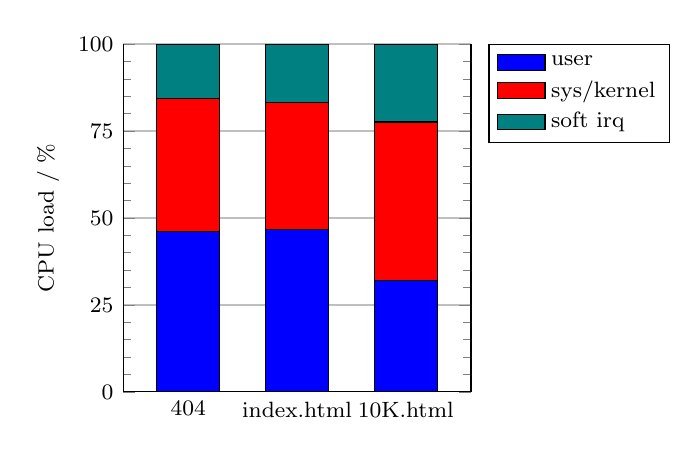
\begin{tikzpicture}
		\begin{axis}[ybar stacked,
			legend style={at={(1.05,1.0)},anchor=north west},
			xtick={0,1,2},
			axis x line*=bottom,
			tick label style={font=\footnotesize},
			legend style={font=\footnotesize},
			label style={font=\footnotesize},
			ytick={0,25,50,75,100},
			width=6cm,
			height=6cm,
			bar width=8mm,
			ylabel={CPU load / \%},
			xticklabels={404, index.html, 10K.html},
			ymajorgrids=true,
			minor tick style={very thin, gray},
			minor y tick num=4,
			ymin=0,
			ymax=100,
			area legend,
			legend cell align=left,
			enlarge x limits=0.3]
			\addplot[fill=blue] coordinates % usr
			{(0,46.2) (1,46.6) (2,32.1)};
			\addplot[fill=red] coordinates % sys
			{(0,38.1) (1,36.5) (2,45.5)};
			\addplot[fill=teal] coordinates % sirq
			{(0,15.6) (1,16.7) (2,22.3)};
			\legend{user,sys/kernel,soft irq}
		\end{axis}
	\end{tikzpicture}
	\caption{CPU load distribution for different request types.}
  \label{fig:initial-req-cpu}
\end{wrapfigure}

The difference in request and response rates the system can handle is also visible in \textbf{CPU utilization}. Main responsibility of \textit{nginx} for serving requests is to handle the HTTP part of the process. This includes parsing request headers, generating responses and delivering static files. The \gls{os} on the other hand does the "translation" to and from \gls{tcp} and handles all work on lower network layers (see also figure \ref{fig:net-layers}). An increased payload size of single responses entails therefore a shift in processing time from \textit{nginx} ("user space") towards the operations inside the Linux kernel. Figure \ref{fig:initial-req-cpu} shows exactly this correlation.

\clearpage
Network \textbf{throughput} of the tests follows naturally the trend of response rates. For tests requesting the "index.html" file and those resulting in "HTTP 404 -- Not Found" responses, the shown throughput is very low, because \textit{httperf} calculates throughput using the formula $\frac{\text{[size]} \cdot \text{[total repsonses]}}{\text{[test time]}}$. Therefore very small response sizes yield a low average throughput.

\begin{figure}[H]
	\centering
	\begin{tikzpicture}
		\begin{axis}[width=\textwidth,height=6cm,
			xlabel={demanded request rate (per second)},
			ylabel={KB / s},
			extra y tick style={grid=major},
			extra x tick style={grid=major},
			y tick label style={/pgf/number format/1000 sep=},
			minor tick style={very thin, gray},
			minor y tick num=3,
			ymajorgrids=true,
			legend cell align = left,
			legend pos = north west]
			\addplot table[x index=0, y index=13] {graphdata/perf-initial3.csv};
			\addlegendentry{index.html}
			\addplot table[x index=0, y index=14] {graphdata/perf-initial3.csv};
			\addlegendentry{10K.html}
			\addplot table[x index=0, y index=21] {graphdata/perf-initial3.csv};
			\addlegendentry{404}
		\end{axis}
	\end{tikzpicture}
  \caption{Throughput for the different test runs.}
  \label{fig:initial-req-io}
\end{figure}

\subsection{Dedicated Network Throughput Tests}

To test the maximal network throughput the server can provide, a test needs to be designed focusing on just this parameter. This approach prevents other parts of the system from getting into the way. A constant high exchange of TCP packets can be achieved by transferring very few, but large files over the network. Therefore a large binary file having a size of 33.4 MB was used for throughput tests.

Figure \ref{fig:tcp-io-perf} shows the network throughput for requests to this file with an increasing connection rate and two HTTP requests on each connection. The system under test goes into saturation at about 61 Megabits/sec. This is equivalent to $6.1\ \%$ of the available network bandwidth, providing a maximum of 1 Gigabit/sec. It is important to note that the number of 61 Megabits/sec. is not equivalent to the number of actually transferred bits over the network, but only includes the received "usable" data. Transferred connection setup and close, acknowledgment and TCP, IP and Ethernet header messages are not included in this number.

The figure also shows the total CPU utilization of the tested system.

\begin{figure}[H]
	\centering
	\begin{tikzpicture}
		\begin{axis}[width=\textwidth,height=6cm,
			xlabel={connection rate},
			ylabel={$10^6$ bits/s},
			axis  y  line*=left,
			extra y tick style={grid=major},
			extra x tick style={grid=major},
			y tick label style={/pgf/number format/1000 sep=},
			minor tick style={very thin, gray},
			minor y tick num=3,
			ymajorgrids=true,
			legend style = {at={(0.125,-.1)}, anchor=north}]
			\addplot[color=blue,mark=o] table[x index=0, y index=13] {graphdata/tcp-io-perf.csv};
			\addlegendentry{network throughput}
		\end{axis}
		\begin{axis}[width=\textwidth,height=6cm,
			ylabel={percentage},
			axis  y  line*=right,
			axis  x  line=none,
			extra y tick style={grid=major},
			extra x tick style={grid=major},
			y tick label style={/pgf/number format/1000 sep=},
			minor tick style={very thin, gray},
			minor y tick num=3,
			%ymajorgrids=true,
			legend style = {at={(0.93,-.1)}, anchor=north}]
			\addplot[color=red,mark=x] table[x index=0, y index=9] {graphdata/tcp-io-perf.csv};
			\addlegendentry{cpu load}
		\end{axis}
	\end{tikzpicture}
  \caption{Network throughput and CPU load.}
  \label{fig:tcp-io-perf}
\end{figure}

\clearpage
Figure \ref{fig:tcp-io-perf-cpu} shows the CPU utilization by time spent in the different types of the system. It shows that most time is spent in kernel space and handling interrupt requests by the network driver and sub system (soft irq). nginx (user space) takes only very low CPU utilization and is not the limiting factor in this test. This conforms with test results of the previous tests on smaller files.

%usr	%CPU spent by User space applications		
%sys	%CPU spent by the System (kernel mode)		
%nic	%CPU spent by Low priority user mode (nice)		
%Idle	%CPU which is available (idle)		
%io		%CPU spent by I/O waiting		
%irq	%CPU spent servicing interrupt requests		
%sirq	%CPU spent servicing soft irqs	

\begin{figure}[H]
	\centering
	\begin{tikzpicture}
		\begin{axis}[ybar stacked,width=\textwidth,height=6cm,
			xlabel={connection rate},
			ylabel={percentage},
			extra y tick style={grid=major},
			extra x tick style={grid=major},
			y tick label style={/pgf/number format/1000 sep=},
			minor tick style={very thin, gray},
			minor y tick num=3,
			ymajorgrids=true,
			bar width=10mm,
			area legend,
			legend columns=6,
			legend style = {at={(0.5,1.03)}, anchor=south}]
%			legend pos = south east]
			\addplot[fill=red] table[x index=0, y index=2] {graphdata/tcp-io-perf.csv};	%,mark=x
			\addlegendentry{user space  }
			\addplot[fill=blue] table[x index=0, y index=3] {graphdata/tcp-io-perf.csv};	%,mark=o
			\addlegendentry{system/kernel}
%			\addplot[color=magenta,mark=o] table[x index=0, y index=4] {graphdata/tcp-io-perf.csv};
%			\addlegendentry{low priority (nice)}
%			\addplot table[x index=0, y index=5] {graphdata/tcp-io-perf.csv};
%			\addlegendentry{idle}
%			\addplot[color=orange,mark=triangle] table[x index=0, y index=6] {graphdata/tcp-io-perf.csv};
%			\addlegendentry{io (waiting)}
%			\addplot[color=green,mark=|] table[x index=0, y index=7] {graphdata/tcp-io-perf.csv};
%			\addlegendentry{irq}
			\addplot[fill=teal] table[x index=0, y index=8] {graphdata/tcp-io-perf.csv};	%,mark=diamond
			\addlegendentry{soft irq}
		\end{axis}
	\end{tikzpicture}
  \caption{CPU utilization by category.}
  \label{fig:tcp-io-perf-cpu}
\end{figure}

To proof that obtained performance limits were not limits of the client executing the tests or the network infrastructure, the same test was also executed against a "reference system" running a \textit{Microsoft IIS 7.5} web server. Figure \ref{fig:tcp-io-perf-iis} shows the results. Measured throughput (averaged per request) had a maximum at about 515.7 Megabits/sec which outplays the results of the \textit{MicroBlaze} system by more than a factor of eight.

\begin{figure}[H]
	\centering
	\begin{tikzpicture}
		\begin{axis}[width=\textwidth,height=6cm,
			xlabel={connection rate},
			ylabel={$10^6$ bits/s},
			extra y tick style={grid=major},
			extra x tick style={grid=major},
			y tick label style={/pgf/number format/1000 sep=},
			minor tick style={very thin, gray},
			minor y tick num=3,
			ymajorgrids=true,
			legend pos = south east]
			\addplot table[x index=0, y index=15] {graphdata/tcp-io-perf.csv};
			\addlegendentry{network throughput}
		\end{axis}
	\end{tikzpicture}
  \caption[Network throughput of a reference system]{Network throughput of an AMD Phenom II X4 processor at 3.40 GHz running Microsoft IIS 7.5 on Windows 7.}
  \label{fig:tcp-io-perf-iis}
\end{figure}

\section{Discussion of Results}

Obtained performance results show that the designed System on Chip with custom configured and compiled Linux kernel is capable of running a web server serving up to about 300 requests per second and 100 concurrent connections. Compared to the low performance indicator of 48.94 BogoMIPS\footnote{"The number of million times per second a processor can do absolutely nothing." (untraceable source: Eric S Raymond, Geoff Mackenzie -- \url{http://www.tldp.org/HOWTO/html\_single/BogoMips/})}, which is less than a $\frac{1}{130}$ of the value Linux kernel reports for a virtualized \textit{AMD Phenom II X4} processor at 3.40 GHz running on two cores\footnote{6414.98 BogoMips}, this is not to bad. But the capacity of the server would not be sufficient for running it as a public web server connected to the global internet infrastructure. Especially because response rates rapidly decrease with increasing byte size of responses, reasoned in a larger amount of TCP packets required for transmitting the response.

A reduction in the number of TCP packets could be achieved by using so called "Jumbo Frames". These are Ethernet frames with a data size larger than the default \gls{mtu} of 1500 bytes. The responsible setting can be changed executing the command "\texttt{ifconfig eth0 mtu [new size]}". Where \texttt{[new size]} is the new \gls{mtu} size in bytes. Unfortunately this does not seem to be fully supported by the \textit{Xilinx LL TEMAC} Ethernet driver\footnote{see Xilinx forum: \url{http://forums.xilinx.com/t5/Embedded-Linux/Jumbo-frames-ifconfig-crash-and-xps-ll-temac-issues/td-p/211911} (as of 12/2012)}, leading to TCP packets with a total size larger than 1500 bytes to be corrupted and therefore lost "on the network". Besides this, Jumbo Frames would have to be supported on the client and all intermediate stations as well, which can not be guaranteed on a public network or on providing a public service.

\textit{nginx} provides a configuration setting "\texttt{worker\_connections}" which limits the maximum amount of concurrently handled connections by a worker process. During tests this setting had a value of 768. But neither changing the number of maximum allowed connection to 1024 nor 512 had any influence in observed response rates. Therefore it is safe to be assumed that no internal limit for concurrent connections affected the test results. But therefore this part does not have any room for improvements, either.

Especially the tests for maximum network throughput showed that the main bottleneck is in the TCP and network stack on the test system. Besides providing more processing power to the system, optimizing this part of the Linux kernel is hardly possible in the project context. Another option would be to offload processing of TCP connections, requests and responses to dedicated hardware, implemented as a network interface with enhanced functionality. This possible solution is also refereed to by the title of this thesis using the word "accelerated", but requires deep integration into already available functions of the operating system. Therefore the next two chapters will provide an overview of the Linux network stack and possible integration options for a \textit{TCP Offload Engine} (TOE).